% Generated by scripts/flatten_paper.py from paper/main.tex. Do not edit; edit the sources.
\documentclass[conference]{IEEEtran}
\IEEEoverridecommandlockouts

\usepackage{cite}
\usepackage{amsmath,amssymb,amsfonts}
\usepackage{algorithmic}
\usepackage{graphicx}
\usepackage{textcomp}
\usepackage{xcolor}
% Added for the generated result tables and links.
\usepackage{iftex}
\ifXeTeX
  % XeTeX/Tectonic builds lack the Type-1 Times that IEEEtran uses under pdfLaTeX.
  \usepackage{fontspec}
  \setmainfont{texgyretermes}[Extension=.otf, UprightFont=*-regular, BoldFont=*-bold,
    ItalicFont=*-italic, BoldItalicFont=*-bolditalic]
\fi
\usepackage{booktabs}
\usepackage{array}
\usepackage{url}
\usepackage[hidelinks]{hyperref}

\def\BibTeX{{\rm B\kern-.05em{\sc i\kern-.025em b}\kern-.08em
T\kern-.1667em\lower.7ex\hbox{E}\kern-.125emX}}

% Visible placeholder for anything the team still has to check or decide.
% The submitted version must compile with zero \todo occurrences.
\newcommand{\todo}[1]{\textcolor{red}{[TODO: #1]}}

\begin{document}

% ============================================================
% TITLE
% ============================================================

\title{
Continual Learning for Adaptive Health and Reuse Assessment of
Heterogeneous Second-Life EV Batteries
}

% ============================================================
% AUTHORS
% ============================================================

\author{
\IEEEauthorblockN{Tarun Sitaraman}
\IEEEauthorblockA{
\textit{Department of Networking and}\\
\textit{Communications}\\
\textit{SRM Institute of Science}\\
\textit{and Technology}\\
Chennai, India\\
RA2411028010038
}
\and
\IEEEauthorblockN{Sohan Sandeep Krishnan}
\IEEEauthorblockA{
\textit{Department of Networking and}\\
\textit{Communications}\\
\textit{SRM Institute of Science}\\
\textit{and Technology}\\
Chennai, India\\
RA2411028010014
}
\and
\IEEEauthorblockN{Darshan D}
\IEEEauthorblockA{
\textit{Department of Networking and}\\
\textit{Communications}\\
\textit{SRM Institute of Science}\\
\textit{and Technology}\\
Chennai, India\\
RA2411028010056
}
}

\maketitle

% ============================================================
% ABSTRACT
% ============================================================

\begin{abstract}
Retired electric-vehicle batteries can serve in second-life applications, but a health model trained on one battery population may fail on the next, and continual learning promises to adapt without forgetting. We test this promise for forecasting the state of health (SOH) of lithium-ion cells one to six capacity checks ahead, on a leakage-controlled benchmark from five public datasets (395 cells), with follow-up experiments pre-registered and every claimed difference replicated on a second seed set. A Temporal Fusion Transformer with Elastic Weight Consolidation (TFT\,+\,EWC) is compared with fine-tuning, replay, joint training, literature backbones and simple forecasters. Forgetting appears whenever usage conditions differ (0.18--0.46 percentage points, pp). Trained on a shrunk correction to linear extrapolation, TFT\,+\,EWC matches extrapolation on the continual stream and beats it by 0.12--0.20~pp on unseen usage conditions, where, however, gradient boosting is 0.39--0.60~pp more accurate and the same TFT trained jointly beats its continual form by 0.32--0.44~pp. Shift-adaptive EWC, first-life pretraining and Spark-extracted inputs from 0.9 billion ageing measurements do not help. Conformal intervals calibrated on the training conditions under-cover on unseen ones (0.66--0.76 at 90\%); calibrating on conditions held out from fitting restores 0.90 coverage, except on a condition outside the training range (0.38--0.48). With these intervals, 87--92\% of forecasts fall within one reuse class, over 99\% of them correctly.
\end{abstract}

% ============================================================
% KEYWORDS
% ============================================================

\begin{IEEEkeywords}
Continual learning, second-life batteries, electric vehicles, state of health, battery degradation, heterogeneous batteries, catastrophic forgetting, machine learning
\end{IEEEkeywords}

% ============================================================
% I. INTRODUCTION  (team draft, condensed to the IEEE conference length)
% ============================================================

\section{Introduction}

When an electric-vehicle (EV) battery no longer meets automotive requirements, it may still serve less demanding applications such as stationary storage or backup power. Reuse extends the battery's life and delays recycling, but only if its health is assessed reliably.

The state of health (SOH) describes the present capability of a battery relative to a reference condition, and machine-learning models have estimated it from voltage, current, temperature, partial charging and impedance measurements~\cite{ref1,ref2,ref3,ref4}. Retired batteries are, however, heterogeneous: chemistry, manufacturer, capacity, first-life history, temperature and charging protocol differ, and complete first-life records are often missing. A model trained once on a fixed population may therefore fail on the next population. Continual learning addresses this by updating a model on new data while preserving what it learned earlier; it must therefore be evaluated both on the newly introduced battery group and on the groups learned before, to measure catastrophic forgetting.

This work combines continual learning, health assessment and second-life reuse assessment. Health is assessed by \emph{forecasting} the SOH one to six capacity checks ahead from everything measured up to the latest check: on the first dataset studied, estimating the current SOH from cycling features was beaten by carrying the last measured SOH forward (\S\ref{sec:methods}), whereas a reuse decision needs the future SOH. The forecast is mapped to reuse-suitability classes.

The contributions are:
\begin{itemize}
  \item A leakage-controlled benchmark for forecasting the SOH of second-life cells from five public datasets (395 cells after quality rules), with two label artefacts removed: test currents set from the previous capacity, and pulse charge counted in the capacity.
  \item An evaluation of a Temporal Fusion Transformer with Elastic Weight Consolidation (TFT\,+\,EWC) against fine-tuning, replay, joint training, simple forecasters and the model families of the literature (BiLSTM, TCN, Transformer, GPR, random forest, SVR) under three protocols (a continual stream, unseen groups and first-life pretraining), reporting adaptation, forgetting and retention.
  \item A continual TFT\,+\,EWC that learns a shrunk correction to linear extrapolation: on the continual stream it matches extrapolation, which no model beats, and EWC reduces its forgetting over longer horizons; on unseen usage conditions it beats extrapolation but not gradient boosting or its own jointly trained form (all replicated). Shift-adaptive EWC and first-life pretraining add nothing, null results we report.
  \item Forecast intervals for unseen usage conditions: split-conformal intervals calibrated on the training conditions under-cover, and calibrating on conditions held out from fitting restores nominal coverage over the unseen conditions, except for a condition outside the training range.
  \item A reproducibility analysis showing that several significance results on small battery datasets depend on the numerical environment, and a replication rule that the main results satisfy.
\end{itemize}

% ============================================================
% II. RELATED WORK  (team draft, condensed to the IEEE conference length)
% Bibliographic data of all ten studies verified against Crossref (4 Oct 2026). Figures quoted for
% ref1, ref2, ref4, ref5, ref8 and ref10 were checked against the published abstracts. For ref3, ref6,
% ref7 and ref9 no open abstract was available, so the text states only what their titles state.
% ============================================================

\section{Related Work}

The review covers 2022--2026 studies on second-life lithium-ion batteries, SOH estimation, continual learning and reuse assessment.

\emph{SOH estimation for second life.} Braco \textit{et al.} estimated the SOH of second-life cells from partial charging under residential and fast-charging-station profiles, with offline RMSE of about 0.6 and 0.8\% and 85\% less testing time than a full capacity test~\cite{ref1}. On reused Nissan Leaf modules they compared 58 health indicators; the best reached about 0.2\% RMSE at repurposing, but the most useful indicators changed as ageing progressed~\cite{ref2}. Faraji-Niri \textit{et al.} accelerated second-life SOH estimation with impedance spectroscopy and machine learning~\cite{ref3}. Takahashi \textit{et al.} screened batteries for second life with statistical current and voltage features and bagged Gaussian process regression, with root-mean-squared percent error below 1.48\% in the worst cases~\cite{ref4}. Cui \textit{et al.} tested retired Nissan Leaf cells for more than 15 months under grid-storage-like operation and estimated health online with clustering, with mean absolute percentage error below 2.3\%~\cite{ref5}. Vignesh \textit{et al.} reviewed SOH estimation methods for second-life batteries and their challenges~\cite{ref6}. These studies estimate the \emph{current} SOH of a fixed population; none adapts a model as new, different populations arrive.

\emph{Continual learning and generalisation.} Lee \textit{et al.} applied bilevel-optimised continual learning to predict the capacity degradation of lithium-ion batteries~\cite{ref7}. Yao \textit{et al.} used progressive neural networks with temporal convolutional networks for online state-of-charge estimation across three drive-cycle datasets, addressing catastrophic forgetting and task order~\cite{ref8}. Li \textit{et al.} proposed domain-generalised SOH estimation for second-life EV batteries~\cite{ref9}, and Meskine \textit{et al.} compared BiLSTM, TCN and probabilistic TCN-GPR models on sparse, noisy data, where isotonic recalibration substantially reduced the calibration error~\cite{ref10}. Transfer and domain generalisation do not by themselves address a long sequence of tasks with explicit retention.

\emph{Research gap.} Second-life SOH estimation, screening, transfer learning and degradation prediction have progressed largely separately; continual learning is rarely combined with heterogeneous second-life SOH forecasting, an explicit reuse decision and an evaluation of forgetting. This work asks whether a continual learner can learn heterogeneous second-life populations in sequence while retaining earlier ones, and whether its forecasts support reuse decisions.

% =============================================================================
% Methodology (condensed to the IEEE conference length)
%
% Written from the implementation and docs/DECISIONS.md (D11, D12, D14, D16-D21).
% Data sources: docs/EXTERNAL_DATA.md. Every number in this section is traceable
% to results/*.json on a clean commit or to the data report (docs/DATA_REPORT.md).
% The full protocol, feature lists and data-quality rules are in the repository.
% =============================================================================

\section{Methodology}
\label{sec:methods}

Given everything measured up to a reference performance test (RPT, or capacity check), we forecast the SOH one to three checks ahead, and up to six in the follow-up experiments. Cells or usage conditions arrive as a stream of tasks, and a model must adapt to each new task without forgetting the earlier ones.

\emph{Change of task after inspecting the data.} The study was first designed to estimate the \emph{current} SOH from cycle-level features. On the first dataset these features carried almost no health information (median within-cell Spearman correlation with SOH 0.09, against $-0.99$ for elapsed time), and learned estimators were worse than persistence (1.78 and 2.37~pp for gradient boosting and ridge regression, against 0.99~pp). We therefore reframed the task as forecasting after seeing the data, and committed the forecasting protocol before fitting any forecasting model.

% -----------------------------------------------------------------------------
\subsection{Datasets}
\label{sec:data}

Table~\ref{tab:data} lists the five public datasets (all CC~BY~4.0). Every file is verified against its repository record or checksums, and our parsing of the raw files reproduces exactly the RPT capacities of the processed S1 tables and the authors' capacities of all 843 S6 checks.

\begin{table}[t]
  \centering
  \caption{Datasets. S1 and S6 form the continual-learning streams; S7--S9 form the first-life pretraining pool.}
  \label{tab:data}
  \scriptsize
  \setlength{\tabcolsep}{2.5pt}
  \begin{tabular}{p{0.95cm}p{3.0cm}p{1.75cm}r}
    \toprule
    Set & Cells and conditions & Label & Samples \\
    \midrule
    S1~\cite{moy2024secondlife,moy2024secondlifedata} & 6 NMC 21700 cells, second life on residential or commercial peak shaving, 20/35~$^\circ$C blocks & C/20 RPT capacity, pulses excluded & 279 \\
    S6~\cite{wheeler2025lfp,wheeler2025lfpdata} & 20 LFP 18650 cells, 7 conditions (charge mode, voltage and rate, discharge, depth), 50~$^\circ$C & C/25 check capacity & 2{,}409 \\
    S7~\cite{luh2024agingdata,luh2024agingdatav2} & 195 of 228 NMC/C+SiO cells, calendar, cyclic and WLTP ageing, 0--40~$^\circ$C & check-up capacity & 10{,}251 \\
    S8~\cite{wang2024pinn,wang2024pinndata} & 55 NCM cells, six charge/discharge protocols & capacity cycles & 9{,}699 \\
    S9~\cite{zhu2022relaxation,zhu2022relaxationdata} & 119 of 130 NCA, NCM and blended cells, 25--45~$^\circ$C & capacity cycles & 16{,}761 \\
    \bottomrule
  \end{tabular}
\end{table}

\emph{S1} contains six LG~Chem INR21700-M50T cells that spent 23 months under an EV driving profile~\cite{pozzato2022firstlife} and then about 27 months on peak-shaving duty cycles~\cite{moy2023dutycycles}; each RPT is a C/20 discharge interrupted by C/2 pulses, with impedance spectroscopy (EIS) from the fifth RPT~\cite{moy2024secondlife}. Data-quality findings are handled by fixed rules (e.g.\ RPT~2, run at about 20~$^\circ$C, is excluded).

\emph{S6} was selected by criteria fixed before screening (licence, a capacity-check series, ageing past first-life end of life, heterogeneity that S1 lacks). Its cells were characterised every 100 cycles and end at 32--64\% SOH; ``second life'' here means continued ageing below 80\% SOH under the same protocol. A check is used only if its C/25 discharge starts from full charge and reaches the cut-off (843 of 847 checks).

\emph{S7--S9} are first-life datasets used for pretraining. Cells with at least five valid checks are kept: 369 cells and 36{,}711 samples.

\subsection{Big-data processing of the ageing cycles}
\label{sec:spark}

Between checks, every S6 cell logged each ageing cycle at about one sample per second: 827 files, 132~GB raw and $9.0\times10^{8}$ rows. Apache Spark~4.2 (PySpark, local mode) reduces them to block-level inputs. One map task per 100-cycle block derives, for every cycle, a validity flag and seven measured responses (end-of-charge and end-of-discharge voltage, constant-voltage hold time and final current, relaxation after charge and after discharge, internal resistance); Spark SQL groups the cached per-cycle table (82{,}529 cycles) by cell and block into the mean, last value and slope of each response (21 inputs), and each block joins the origin at the check that ends it. Charge, energy and current are excluded because the protocol scales them with the previous capacity (within-cell $r=0.97$--$0.999$ with the previous check's capacity). The full run takes 20~min on six cores, and its output matches an independent pandas implementation on all 827 blocks (largest difference $2\times10^{-13}$).

\subsection{State of health and forecasting target}
\label{sec:soh}
\label{sec:task}
\label{sec:features}

For cell $b$ with check capacities $C_{b,1}, C_{b,2},\dots$ in time order,
\begin{equation}
  \mathrm{SOH}_{b,k} = 100\,C_{b,k}/C_{b,1}\;\%,
  \label{eq:soh}
\end{equation}
i.e.\ relative to the first valid measurement, not to a nominal rating. In S1 the capacity is the charge of the C/20 steps only~\cite[Eq.~(1)]{moy2024secondlife}; the processed tables we started from also counted the pulse charge, which shifts some labels by up to 0.09~pp.

A sample is a triple (cell $b$, origin $k$, horizon $h\in\{1,2,3\}$), about one to three months in S1 and 100--300 cycles in S6. The target is
\begin{equation}
  \Delta_{b,k,h} = \mathrm{SOH}_{b,k+h} - \mathrm{SOH}_{b,k},
  \label{eq:target}
\end{equation}
so an error in $\Delta$ equals the error in the future SOH; errors are root-mean-square errors (RMSE) in SOH percentage points (pp). The fade rate $r_{b,k}$ is the least-squares slope of SOH against time $t$ (days or cycles) over the last three valid checks,
\begin{equation}
  r_{b,k} = \frac{\sum_{i=k-2}^{k} (t_{b,i}-\bar t)(\mathrm{SOH}_{b,i}-\overline{\mathrm{SOH}})}{\sum_{i=k-2}^{k} (t_{b,i}-\bar t)^2}.
  \label{eq:fade}
\end{equation}

Inputs use only information available at the origin. \textbf{F0} contains the SOH history ($\mathrm{SOH}_{b,k}$, time or cycles since the first check, $r_{b,k}$), static descriptors (S1: duty cycle and first-life history~\cite{moy2024secondlife}; S6: test conditions) and the \emph{planned} usage until the target (S1: days at each temperature set point and at rest; S6: cycles), so forecasts are conditional on the planned usage. \textbf{F1} adds diagnostics measured at the origin: 47 in S1 (pulse resistances, incremental-capacity and EIS features) and 17 in S6 (plateau charges, incremental-capacity peaks, hysteresis, a resistance proxy). No test current is an input: in S1 the RPT and monthly discharge currents were set from the previous capacity and therefore encode the label. Missing values are imputed from training data and flagged.

\subsection{Splits and protocols}
\label{sec:protocols}

\emph{Purged chronological splits.} For each cell, cut~A lies at 60\% and cut~B at 80\% of its valid checks. Training samples have their target at or before~A, validation samples their origin at or after~A and target at or before~B, and test samples their origin at or after~B; samples straddling a cut are dropped, so no training label lies after a validation origin and no validation label after a test origin.

\emph{P1, continual stream.} A task is a cell in S1 (six tasks) or a test condition in S6 (seven tasks). At step $i$ of an ordering $\pi$, a strategy receives only task $\pi_i$'s data. Each method runs on 10 orders with 5 seeds, identical across methods.

\emph{P2, unseen group.} One cell (S1) or condition (S6) is held out; models are trained on the others and tested on all its samples.

\emph{P3, first-life pretraining.} All datasets are mapped onto shared inputs (SOH history, calendar and cycle time, planned time to the target, operating conditions and chemistry, undefined conditions flagged as missing). Models are pretrained on the pool, which also supplies the input scaling and the first EWC anchor, and the seven S6 conditions then follow as a stream.

\subsection{Models}
\label{sec:backbones}

Preprocessing (standardisation, median imputation with missing indicators, target scaling) is fitted on the first task and then frozen. The \emph{MLP} has hidden layers of 128 and 64 ReLU units (dropout 0.1). The proposed backbone adapts the Temporal Fusion Transformer (TFT)~\cite{lim2021tft}: a window of the $W{=}4$ most recent origins of the same cell and horizon (inputs only, never labels) passes through per-variable embeddings, variable selection by gated residual networks, an LSTM encoder~\cite{hochreiter1997lstm} and interpretable two-head attention masked to past steps.

\emph{Strategies.} Fine-tuning trains on the current task only (lower bound); experience replay~\cite{rolnick2019replay} stores $B$ samples per finished task; joint training fits all tasks at once (upper bound); and Elastic Weight Consolidation (EWC)~\cite{kirkpatrick2017ewc} adds, for each finished task $j$,
\begin{equation}
  \frac{\lambda}{2}\sum_{p} F_{j,p}\,\big(\theta_p - \theta^{*}_{j,p}\big)^2,
  \label{eq:ewc}
\end{equation}
with $\theta^*_j$ the parameters after task $j$ and $F_j$ the empirical diagonal Fisher information over up to 500 training samples. \emph{TFT\,+\,EWC} is the proposed model. Training uses Adam~\cite{kingma2015adam}, batches of 64, at most 200 epochs and early stopping on the current task's validation RMSE.

\emph{Reference forecasters} are persistence ($\hat\Delta=0$), linear extrapolation $\hat\Delta_{b,k,h} = r_{b,k}(t_{b,k+h}-t_{b,k})$, ridge regression (on planned usage only, F0 or F1) and histogram gradient boosting on F1.

\emph{Learned residual.} Because linear extrapolation proved hardest to beat, a follow-up experiment, specified and committed before it was run, trains the continual learners on the correction to it. With $\hat\Delta^{\mathrm{lin}}_{b,k,h}$ the extrapolation above (zero when $r_{b,k}$ is missing), the model $g_\theta$ learns $\Delta_{b,k,h}-\hat\Delta^{\mathrm{lin}}_{b,k,h}$ and the forecast is
\begin{equation}
  \hat\Delta_{b,k,h} = \hat\Delta^{\mathrm{lin}}_{b,k,h} + g_\theta(\mathbf{x}_{b,k,h}).
  \label{eq:residual}
\end{equation}
The residual and the direct (target $\Delta$) forms are compared on the S6 stream with the P3 shared inputs, from scratch, for horizons 1--3 (E1) and 1--6 (E2).

\emph{Shift-adaptive EWC and literature backbones.} A second pre-registered experiment tests whether the EWC strength should follow the shift between groups. \emph{RC-TFT} trains the residual TFT with shift-adaptive EWC (SA-EWC): when task $t$ starts, the penalty~\eqref{eq:ewc} of each finished task $j$ is multiplied by $d_{j,t}=\big((\lVert\mu_t-\mu_j\rVert^2+\lVert\sigma_t-\sigma_j\rVert^2)/D\big)^{1/2}$, the per-dimension 2-Wasserstein distance between diagonal Gaussians fitted to the two tasks' preprocessed training inputs, with $\lambda_0$ tuned as $\lambda$. Alongside, BiLSTM~\cite{ref10}, TCN~\cite{ref8,ref10} and Transformer-encoder continual learners (the TFT's input window, within 20\% of its 12{,}708 parameters) and single-fit GPR~\cite{ref3,ref4}, random forest and SVR regressors are run in residual and direct form.

\emph{Shrinkage and forecast intervals.} A third pre-registered experiment calibrates the residual model after training, without changing its weights. Per horizon $h$, the learned correction is shrunk towards extrapolation by $\alpha_h=\min\!\big(1,\max(0,\sum p\,y/\sum p^2)\big)$, with $p$ the predicted and $y$ the observed correction on calibration rows. A split-conformal interval~\cite{lei2018conformal} $\hat\Delta\pm q_h$ takes as $q_h$ the $\lceil (n+1)(1-a)\rceil$-th smallest of the $n$ absolute calibration residuals at horizon $h$. Intervals at level $1-a$ (90\% and 80\%) are scored by coverage, width and the interval score~\cite{gneiting2007scoring} $2q_h + \tfrac{2}{a}\max(|\Delta-\hat\Delta|-q_h,0)$ (pp; lower is better). On the stream, both are refitted after each task on its validation rows, and extrapolation gets intervals in the same way.

\emph{Unseen conditions.} A fourth experiment repeats P2 on S6 for the shrunk residual TFT\,+\,EWC: it is streamed over the six training conditions in the ten evaluation orders with the P1 tuned values, and shrinkage and intervals are fitted once on the pooled validation rows of those conditions. Origins with a fade rate (H$^+$) and without (H$^-$, a cell's first two checks, where extrapolation is persistence) are reported separately. A fifth experiment calibrates intervals by leaving one condition out: each training condition is predicted by a model fitted on the other five, and the absolute residuals at all its origins, pooled over the six conditions, give $q_h$, a cross-conformal variant~\cite{barber2021jackknife}, optionally per horizon and stratum (Mondrian). Its forecaster is gradient boosting, the most accurate in P2; being deterministic, it must show a result in both horizon sets instead of two seed sets.

\subsection{Hyperparameters, metrics and statistics}
\label{sec:tuning}
\label{sec:metrics}

Hyperparameters are chosen on validation data from tuning orders disjoint from the evaluation orders: the learning rate per backbone (lowest validation plasticity of fine-tuning streams), then replay $B\in\{50,\dots,400\}$ and EWC $\lambda\in\{10^0,\dots,10^5\}$, extended at a grid edge. From P3 on, ten tuning orders and the one-standard-error rule (the smallest grid value within one standard error of the best) are used.

After each step $i$, every task's test set is evaluated, giving $R_{i,j} = \mathrm{RMSE}(\mathcal{D}^{\mathrm{te}}_{\pi_j}\mid\theta_i)$. Following~\cite{lopezpaz2017gem,chaudhry2018rwalk}, we report the final average error $\tfrac{1}{T}\sum_{j} R_{T,j}$, backward transfer $\tfrac{1}{T-1}\sum_{j<T} (R_{T,j} - R_{j,j})$ and forgetting $\tfrac{1}{T-1}\sum_{j<T} (R_{T,j} - \min_{j\le i<T} R_{i,j})$ (positive values mean forgetting), the skill $1-\mathrm{RMSE}/\mathrm{RMSE}_{\mathrm{persistence}}$, and the agreement of the reuse class of the forecast SOH with the measured class (C0 $>95\%$, C1 90--95\%, C2 80--90\%, C3 $\le80\%$, fixed in advance).

Means carry 95\% bootstrap intervals~\cite{efron1993bootstrap}. Methods are compared by two-sided Wilcoxon signed-rank tests~\cite{wilcoxon1945} on matched runs or held-out groups, with rank-biserial effect sizes~\cite{kerby2014rankbiserial} and Holm correction~\cite{holm1979}. A difference $d$ is \emph{replicated} only if it is significant in the main seed set (0--4) and in a replicate set (5--9), with the same sign and $|d|\ge 0.05$~pp in both; $|d|<0.05$~pp in both means practically equivalent. The threshold is about half the label shift caused by the pulse-charge definition.

\subsection{Implementation and availability}
\label{sec:repro}

The pipeline uses Python~3.11, NumPy~2.4, pandas~3.0, scikit-learn~1.9 and PyTorch~2.14.1 (P1 and P2 were first run on an Intel Xeon with an unrecorded PyTorch version and re-run on an Intel Core~5~210H), with one CPU thread and seeded, deterministic algorithms. Every result file records configuration, seeds, library versions and the Git commit; unit tests cover input causality, split purging and the exclusion of labels from the inputs. The datasets are at doi:10.17605/OSF.IO/8JNR5 (S1), 10.57745/OLBXKT (S6), 10.35097/1969 (S7), 10.5281/zenodo.10963339 (S8) and 10.5281/zenodo.6405084 (S9); code, decision log and results are kept in a private repository and are available from the authors on request.

% =============================================================================
% Results (condensed to the IEEE conference length)
%
% Numbers are from committed results files produced on clean commits:
% results/forecasting.json (S1, d710cad), results/forecasting_wheeler.json (S6,
% 53ab76f), their re-runs (docs/RESULTS.md, Reproducibility check),
% results/forecasting_d21_p3.json (57e37aa), results/forecasting_d21_ablation_a1*.json
% and results/d21_tft_interpretation.json; D23 and D24 from
% results/forecasting_d23_e*.json (5ae2f84) and results/forecasting_d24_e*.json (947b33a); D25-D27 from
% results/forecasting_d25_e*.json (a59debb), results/forecasting_d26_e*.json (9866d7a) and
% results/forecasting_d27_e*.json (494b36f), summarised in docs/RESULTS.md; table d26 is written
% from those files by hand. Other tables are generated by scripts/make_results_tables.py; figures by
% scripts/make_d25_d27_figures.py.
% =============================================================================

\section{Results}
\label{sec:results}

\emph{Data.} S1 diagnostics track the current SOH (median within-cell $\rho=0.97$ for the main incremental-capacity peak) but not the change to the next RPT (median $|\rho|\le0.3$); every S1 sample stays in class C0, while all S6 cells cross from C0 to C3.

% -----------------------------------------------------------------------------
\subsection{Continual stream (P1)}
\label{sec:res-p1}

% Generated by scripts/make_results_tables.py from results/forecasting.json (commit d710cad), results/forecasting_wheeler.json (commit 53ab76f)
\begin{table*}[t]
  \centering
  \caption{Protocol P1 (continual stream). Final average test RMSE of SOH$(k{+}h)$ in pp (mean $\pm$ s.d.\ over 10 orders $\times$ 5 seeds for continual methods, over 5 seeds for joint training), skill relative to persistence ($1-\mathrm{RMSE}/\mathrm{RMSE}_{\mathrm{persistence}}$) and forgetting (pp). $^\dagger$Upper bound, trained on all tasks at once.}
  \label{tab:p1}
  \begin{tabular}{lccc|ccc}
    \toprule
    & \multicolumn{3}{c|}{S1: six NMC second-life cells} & \multicolumn{3}{c}{S6: 20 LFP cells, seven usage conditions} \\
    Method & RMSE & Skill & Forgetting & RMSE & Skill & Forgetting \\
    \midrule
    Persistence & 0.632 & 0.00 & -- & 1.644 & 0.00 & -- \\
    Linear extrapolation & 0.726 & -0.15 & -- & 0.343 & 0.79 & -- \\
    Ridge, usage only & 0.450 & 0.29 & -- & 1.274 & 0.22 & -- \\
    Ridge, F0 & 0.678 & -0.07 & -- & 0.801 & 0.51 & -- \\
    Ridge, F1 & 0.491 & 0.22 & -- & 0.605 & 0.63 & -- \\
    Gradient boosting, F1 & 0.466 & 0.26 & -- & 0.372 & 0.77 & -- \\
    \midrule
    MLP fine-tuning & 0.492 $\pm$ 0.029 & 0.22 & 0.030 & 0.531 $\pm$ 0.151 & 0.68 & 0.207 \\
    MLP replay & 0.475 $\pm$ 0.021 & 0.25 & 0.025 & 0.597 $\pm$ 0.178 & 0.64 & 0.212 \\
    MLP + EWC & 0.497 $\pm$ 0.033 & 0.21 & 0.040 & 0.540 $\pm$ 0.176 & 0.67 & 0.212 \\
    MLP joint$^\dagger$ & 0.500 $\pm$ 0.016 & 0.21 & -- & 0.414 $\pm$ 0.037 & 0.75 & -- \\
    \midrule
    TFT fine-tuning & 0.467 $\pm$ 0.014 & 0.26 & 0.026 & 0.883 $\pm$ 0.538 & 0.46 & 0.461 \\
    \textbf{TFT + EWC} & 0.462 $\pm$ 0.019 & 0.27 & 0.016 & 0.677 $\pm$ 0.261 & 0.59 & 0.274 \\
    TFT + EWC, F0 & 0.472 $\pm$ 0.020 & 0.25 & 0.019 & 0.621 $\pm$ 0.257 & 0.62 & 0.176 \\
    TFT joint$^\dagger$ & 0.455 $\pm$ 0.017 & 0.28 & -- & 0.427 $\pm$ 0.049 & 0.74 & -- \\
    \bottomrule
  \end{tabular}
\end{table*}

Table~\ref{tab:p1} gives the final average error, skill and forgetting.

\emph{S1.} TFT\,+\,EWC reaches 0.462~pp (skill 0.27), level with gradient boosting, TFT fine-tuning and MLP replay (0.466--0.475~pp); a ridge regression on the planned usage alone is slightly better (0.450~pp). Forgetting is small for every method (0.016--0.040~pp). Differences with TFT\,+\,EWC whose significance changed in a re-run are only 0.005--0.014~pp (\S\ref{sec:res-repro}), so we report S1 differences as practically equivalent.

\emph{S6.} When tasks differ in usage, forgetting is substantial (0.18--0.46~pp). EWC lowers the TFT's mean error and forgetting relative to fine-tuning (0.677 against 0.883~pp), but which difference is significant changed between runs (\S\ref{sec:res-repro}). MLP fine-tuning and MLP\,+\,EWC (0.531 and 0.540~pp) are significantly better in both runs, the joint upper bounds (0.414 and 0.427~pp) put the TFT's continual-learning cost at about 0.25~pp, and linear extrapolation (0.343~pp) and gradient boosting (0.372~pp) are the best forecasters. The TFT varies strongly with task order (s.d.\ 0.26~pp with EWC, 0.54~pp with fine-tuning).

% -----------------------------------------------------------------------------
\subsection{Unseen cell or usage condition (P2)}
\label{sec:res-p2}

% Generated by scripts/make_results_tables.py from results/forecasting.json (commit d710cad), results/forecasting_wheeler.json (commit 53ab76f)
\begin{table}[t]
  \centering
  \caption{Protocol P2 (unseen battery in S1, unseen usage condition in S6): mean test RMSE (pp) over held-out groups, range over groups, and for S6 reuse-class accuracy / macro-F1 of the forecast SOH.}
  \label{tab:p2}
  \setlength{\tabcolsep}{3pt}
  \begin{tabular}{llccc}
    \toprule
    Data & Method & RMSE & Range & Class acc./F1 \\
    \midrule
    S1 & Persistence & 0.545 & 0.436--0.688 & -- \\
    S1 & Linear extrapolation & 0.511 & 0.284--0.725 & -- \\
    S1 & Ridge, usage only & 0.301 & 0.172--0.409 & -- \\
    S1 & Ridge, F0 & 0.418 & 0.158--0.779 & -- \\
    S1 & Ridge, F1 & 0.320 & 0.161--0.477 & -- \\
    S1 & Gradient boosting, F1 & 0.219 & 0.091--0.299 & -- \\
    S1 & MLP & 0.285 & 0.149--0.389 & -- \\
    S1 & TFT & 0.292 & 0.199--0.377 & -- \\
    \midrule
    S6 & Persistence & 2.817 & 2.025--4.327 & 0.85 / 0.64 \\
    S6 & Linear extrapolation & 1.372 & 0.856--1.669 & 0.94 / 0.75 \\
    S6 & Ridge, usage only & 1.177 & 0.870--2.288 & 0.95 / 0.83 \\
    S6 & Ridge, F0 & 0.859 & 0.598--1.836 & 0.96 / 0.86 \\
    S6 & Ridge, F1 & 1.137 & 0.588--2.188 & 0.96 / 0.85 \\
    S6 & Gradient boosting, F1 & 0.710 & 0.395--1.839 & 0.97 / 0.88 \\
    S6 & MLP & 0.821 & 0.476--2.225 & 0.96 / 0.87 \\
    S6 & TFT & 0.868 & 0.551--2.390 & 0.96 / 0.88 \\
    \bottomrule
  \end{tabular}
\end{table}

Gradient boosting is best on both datasets (Table~\ref{tab:p2}). On S6 the 100\% depth-of-discharge condition is the hardest for every method (1.8--2.4~pp). The reuse class of the forecast SOH agrees with the measured class for 95--97\% of S6 samples with the learned models (macro-F1 0.83--0.88), against 85\% (0.64) for persistence. With six or seven held-out groups, no difference with the TFT survives Holm correction.

% -----------------------------------------------------------------------------
\subsection{Reproducibility of the comparisons}
\label{sec:res-repro}

P1 and P2 were re-run in a pinned environment on data rebuilt from the raw archives. Every baseline, every P2 result and the ranking of methods reproduced; the neural models moved by at most 0.059~pp. On S1, five Holm-corrected comparisons with TFT\,+\,EWC crossed $p=0.05$. On S6, validation selected EWC $\lambda=1000$ instead of 100 (a 0.008~pp tie), and the error advantage of TFT\,+\,EWC over fine-tuning moved from $p_{\mathrm{Holm}}=0.005$ to 0.060, while its reduction of forgetting moved from 0.050 to 0.008. These findings motivated the ten tuning orders, the one-standard-error rule and the replication rule used from P3 on.

% -----------------------------------------------------------------------------
\subsection{First-life pretraining (P3)}
\label{sec:res-p3}

The pool provides 36{,}711 samples, against 2{,}409 in S6, and validation selected EWC $\lambda=0.01$ for the pretrained TFT. Under the replication rule, EWC and fine-tuning are practically equivalent for the pretrained TFT (differences of 0.015--0.017~pp); both backbones are better from scratch on average (TFT 0.401/0.415~pp against 0.509/0.591~pp pretrained with EWC, significant only in the replicate set); and linear extrapolation (0.343~pp) remains the most accurate method. The S6 stream does not degrade the pool test error (TFT\,+\,EWC: 3.280 to 3.148~pp), but on that split the pretrained models are less accurate than extrapolation (3.001~pp): pretraining does not learn a first-life model worth transferring.

\emph{Why the TFT improved.} A post hoc ablation, repeated on the replicate seeds, explains why the TFT trained from scratch improves from 0.891~pp with the earlier inputs to 0.401~pp with the shared inputs: dropping the 17 diagnostic features lowers the error by 0.17--0.35~pp and adding the calendar time between checks by 0.19--0.31~pp, both replicated at both learning rates ($p_{\mathrm{Holm}}\le0.002$). Its attention over the four previous origins is nearly uniform (0.24--0.26 per lag): the TFT makes little use of its history.
\label{sec:res-interp}

% -----------------------------------------------------------------------------
\subsection{Learned residual on linear extrapolation}
\label{sec:res-residual}

\begin{table}[t]
  \centering
  \caption{Learned residual, shift-adaptive EWC and literature baselines on S6 (stream from scratch): final average test RMSE (pp), mean over 50 runs, main / replicate seed sets, and forgetting (pp) for horizons 1--6. Below the line: single fits on all tasks (not continual) and extrapolation.}
  \label{tab:residual}
  \setlength{\tabcolsep}{2.5pt}
  \scriptsize
  \begin{tabular}{lccc}
    \toprule
    Method & E1: $h{=}1$--3 & E2: $h{=}1$--6 & Forgetting, E2 \\
    \midrule
    \textbf{TFT\,+\,EWC, residual} & \textbf{0.339 / 0.314} & \textbf{0.561 / 0.534} & \textbf{0.093 / 0.086} \\
    RC-TFT (residual, SA-EWC) & 0.343 / 0.321 & 0.548 / 0.564 & 0.066 / 0.084 \\
    TFT fine-tuning, residual & 0.347 / 0.337 & 0.673 / 0.612 & 0.282 / 0.220 \\
    TFT\,+\,EWC, direct & 0.504 / 0.487 & 0.802 / 0.835 & 0.135 / 0.166 \\
    MLP\,+\,EWC, residual & 0.374 / 0.366 & 0.659 / 0.694 & 0.205 / 0.225 \\
    BiLSTM\,+\,EWC, residual & 0.328 / 0.370 & 0.669 / 0.765 & 0.229 / 0.318 \\
    Transformer\,+\,EWC, residual & 0.360 / 0.366 & 0.609 / 0.705 & 0.129 / 0.198 \\
    TCN\,+\,EWC, residual & 0.466 / 0.408 & 0.812 / 0.756 & 0.345 / 0.268 \\
    \midrule
    Linear extrapolation & 0.343 & 0.485 & -- \\
    Gradient boosting & 0.451 & 0.898 & -- \\
    SVR, residual & 0.429 & 0.616 & -- \\
    GPR, direct & 1.374 & 2.073 & -- \\
    \bottomrule
  \end{tabular}
\end{table}

Table~\ref{tab:residual} gives the results of the residual form~\eqref{eq:residual}. The criterion fixed in advance for a positive result, residual TFT\,+\,EWC beating linear extrapolation, was \emph{not} met: the two are practically equivalent for horizons 1--3 (differences of $-0.004$ and $-0.029$~pp), and for horizons 1--6 extrapolation is better on average ($+0.076$ and $+0.049$~pp, not replicated). Per horizon, extrapolation is better at $h=1$ and 2 (replicated), and the gap closes without reversing by $h=5$--6. Learning the residual is, however, what makes the TFT competitive: it improves TFT\,+\,EWC over the direct form by 0.17~pp (E1) and 0.24--0.30~pp (E2) and puts it ahead of gradient boosting, all replicated. With horizons 1--6, where the residual TFT forgets more, EWC lowers its forgetting from 0.28/0.22 to 0.09~pp and its backward transfer from 0.18/0.14 to 0.03~pp, replicated; its effect on the final error is not. For horizons 1--3, EWC and fine-tuning are practically equivalent.

\emph{Ageing-cycle inputs.} Adding the 21 Spark-extracted inputs (Section~\ref{sec:spark}) to the residual TFT\,+\,EWC, as specified before the run, makes it worse: 0.480/0.501 against 0.339/0.314~pp, and worse than linear extrapolation, both replicated.

% -----------------------------------------------------------------------------
\subsection{Shift-adaptive EWC and literature baselines}
\label{sec:res-d24}

Table~\ref{tab:residual} also gives the second pre-registered experiment. The criterion for SA-EWC was \emph{not} met: RC-TFT and the fixed-$\lambda$ residual TFT\,+\,EWC are practically equivalent in final error and forgetting for both horizon sets (differences of at most 0.03~pp), although the shift weights did vary (0.05--1.14), so the simpler fixed-$\lambda$ model remains the best-supported variant. The residual TFT is not uniquely accurate at short horizons: BiLSTM\,+\,EWC (direct, 0.323~pp, and residual) and the residual Transformer\,+\,EWC are practically equivalent to RC-TFT for horizons 1--3. For horizons 1--6, RC-TFT beats the residual BiLSTM and TCN (replicated; the Transformer difference is not replicated). Every single-fit regressor is worse than RC-TFT (replicated), except the residual SVR for horizons 1--6.

% -----------------------------------------------------------------------------
\subsection{Shrinkage and intervals on the stream}
\label{sec:res-d25}

Shrinking the correction per horizon makes the residual TFT\,+\,EWC practically equivalent to extrapolation at every horizon (0.318/0.308 against 0.343~pp for horizons 1--3, 0.498/0.493 against 0.485~pp for 1--6), removing its replicated loss at $h=1$--2; the correction is turned down most at $h=1$ (Fig.~\ref{fig:d25}). This criterion for a positive result was again not met: the model matches extrapolation, it does not beat it. Its 90\% intervals are narrower than extrapolation's but under-cover (0.71--0.81, against 0.92--0.95), so the interval scores are equal (practically equivalent or not replicated). Pretraining the residual model on the first-life pool makes it worse for horizons 1--3 (by 0.22~pp, replicated) and does not help for 1--6.

\begin{figure}[t]
  \centering
  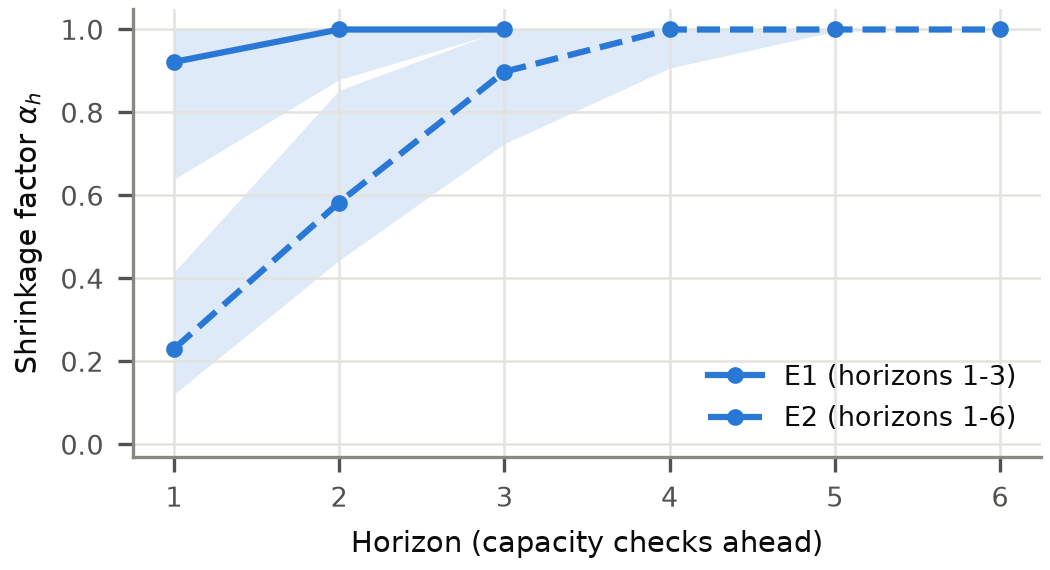
\includegraphics[width=\columnwidth]{figures/d25_shrinkage.png}
  \caption{S6 stream: shrinkage factor $\alpha_h$ of the TFT correction per horizon after the last task (median and interquartile range over 50 runs, seeds 0--4); $\alpha_h=0$ is linear extrapolation.}
  \label{fig:d25}
\end{figure}

% -----------------------------------------------------------------------------
\subsection{Residual model on unseen conditions}
\label{sec:res-d26}

\begin{table}[t]
  \centering
  \caption{Unseen S6 usage condition (P2, seven held-out conditions): test RMSE (pp), mean over folds, on all origins and on origins with a fade rate (H$^+$). TFT rows: mean over 50 runs, main / replicate seed sets; other rows: single deterministic fits.}
  \label{tab:d26}
  \setlength{\tabcolsep}{2.5pt}
  \scriptsize
  \begin{tabular}{lcccc}
    \toprule
    & \multicolumn{2}{c}{E1: $h{=}1$--3} & \multicolumn{2}{c}{E2: $h{=}1$--6} \\
    Method & all & H$^+$ & all & H$^+$ \\
    \midrule
    TFT\,+\,EWC, residual, shrunk & 0.92 / 0.94 & 0.74 / 0.74 & 1.62 / 1.65 & 1.42 / 1.44 \\
    TFT\,+\,EWC, residual, raw & 0.88 / 0.90 & 0.79 / 0.80 & 1.59 / 1.62 & 1.46 / 1.49 \\
    TFT, residual, joint & 0.57 / 0.58 & 0.54 / 0.55 & 1.21 / 1.18 & 1.22 / 1.19 \\
    \midrule
    Gradient boosting & \textbf{0.54} & \textbf{0.51} & \textbf{1.05} & \textbf{1.05} \\
    Ridge & 0.77 & 0.69 & 1.30 & 1.26 \\
    Linear extrapolation & 1.37 & 0.86 & 2.30 & 1.62 \\
    Persistence & 2.82 & 2.66 & 4.90 & 4.73 \\
    \bottomrule
  \end{tabular}
\end{table}

Table~\ref{tab:d26} gives the fourth experiment. As registered, the shrunk residual TFT\,+\,EWC beats extrapolation at origins with a fade rate, by 0.12/0.12~pp for horizons 1--3 and 0.20/0.18~pp for 1--6 (replicated): the first comparison in which the proposed model beats extrapolation. At the other origins extrapolation is persistence and loses by more than 2~pp. Gradient boosting, however, is more accurate than the TFT by 0.39/0.41~pp and 0.57/0.60~pp (replicated), on six of the seven conditions; only on the 100\% depth-of-discharge condition is the TFT better. The same residual TFT trained jointly on the six conditions beats its continual form by 0.32--0.44~pp (replicated). Shrinkage and the raw correction are practically equivalent here. The learning rate and $\lambda$ come from P1 tuning streams that used validation rows of all seven conditions, which can only favour the TFT.

\begin{figure}[t]
  \centering
  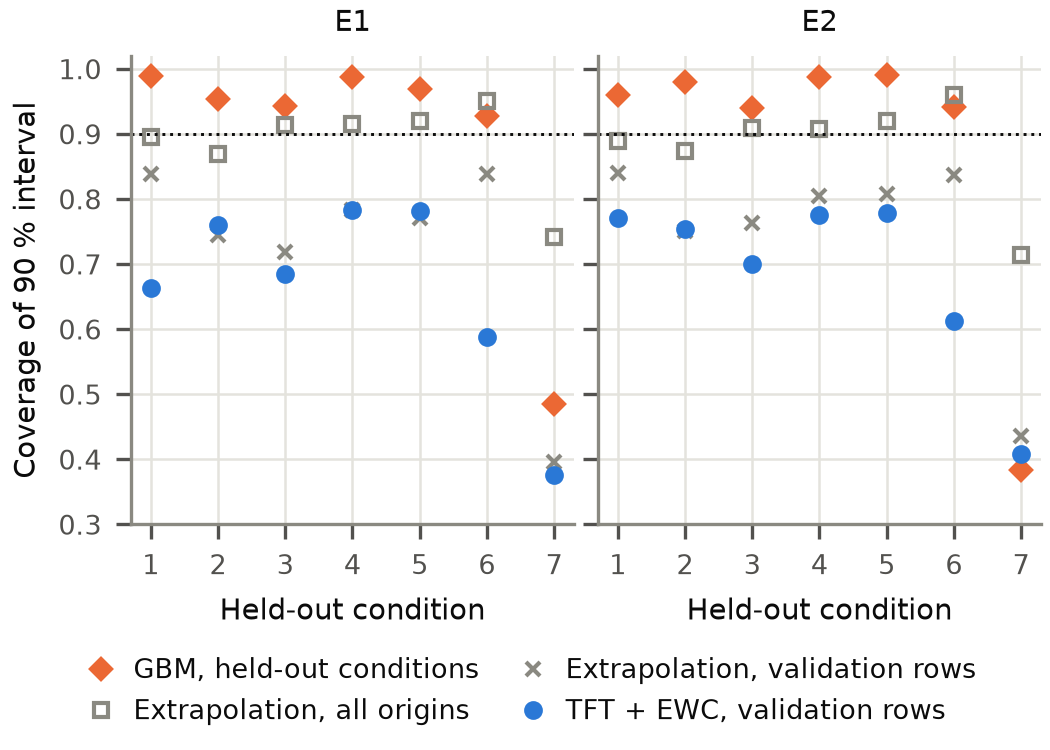
\includegraphics[width=\columnwidth]{figures/d27_coverage.png}
  \caption{Unseen S6 conditions: coverage of 90\% conformal intervals per held-out condition, by forecaster and calibration rows. TFT: mean over 50 runs (seeds 0--4). Dotted: nominal level.}
  \label{fig:d27}
\end{figure}

\emph{Intervals on unseen conditions.} Fig.~\ref{fig:d27} combines the fourth and fifth experiments. Intervals calibrated on the pooled validation rows of the training conditions under-cover on the held-out one, for the TFT (pooled 0.66--0.68) and for extrapolation (0.74--0.76) alike. Calibrating extrapolation, which has no fitted parameters, on all origins of the same conditions instead of their mid-life validation rows restores 0.89--0.90: the calibration rows, not only the model, caused the shortfall. With leave-one-condition-out calibration, gradient-boosting intervals reach the registered threshold of 0.85 (0.90 in both horizon sets) with the lowest mean interval scores (3.2 and 6.7~pp, against 7.1 and 11.8~pp for calibrated extrapolation and 6.1--6.3 and 10.0--10.3~pp for the TFT), lower than calibrated extrapolation's on six of seven conditions (significant for horizons 1--3, $p=0.047$, but not for 1--6, $p=0.30$, so not established). The coverage holds over conditions, not for each: on the 100\% depth-of-discharge condition, which lies outside the range of the others, it is 0.48 and 0.38. Per-stratum half-widths raise extrapolation's coverage at origins without a fade rate from 0.01--0.02 to 0.91--0.92 (interval scores 4.8 and 8.5~pp) and change little for gradient boosting. With these intervals, 87--92\% of held-out forecasts lie within one reuse class, and 99.4--99.7\% of those classes are correct.

% ============================================================
% V. DISCUSSION and VI. CONCLUSION (condensed to the IEEE conference length)
% Every number is taken from docs/RESULTS.md and the committed results files.
% ============================================================

\section{Discussion}
\label{sec:discussion}

\emph{Why the proposed model does not win.} On the continual stream TFT\,+\,EWC never beat linear extrapolation: fade over one to three checks is smooth, leaving little structure for a sequence model to add; the groups are few and small (21--27 and 135--225 training samples per task in S1 and S6); and the TFT barely uses its history. EWC behaves as expected where there is something to protect (forgetting is negligible across the near-identical S1 cells and substantial across the S6 conditions), and its clearest benefit came once the TFT learned only the correction to extrapolation, cutting forgetting over six horizons by about two thirds. Making the penalty follow the measured shift added nothing, plausibly because per-pair weights of 0.05--1.14 matter little next to the choice of $\lambda$ (an interpretation, not tested). The backbone matters less than the target: at horizons 1--3 a BiLSTM or Transformer with EWC is as accurate as the residual TFT. On unseen conditions the continual constraint itself becomes the main cost: trained jointly, the same model is 0.32--0.44~pp more accurate. A model never shown the new condition gains nothing from adapting and still pays for the order of the stream; with datasets this small, storing every earlier group is cheap, so the constraint that motivates continual learning did not bind.

\emph{What matters.} Building on the best simple forecaster mattered most, and the ablation points to the inputs rather than the architecture: the diagnostic features hurt the TFT, and the calendar time between checks helped, consistent with fade per cycle rising with that time at 50~$^\circ$C in all 20 S6 cells. For intervals, the calibration rows mattered as much as the model: residuals from mid-life validation origins of conditions seen in training understate the error on a new condition, while residuals from conditions held out from fitting reproduce it. With few cells per condition, 21 dense ageing-cycle inputs added more variance than information, and first-life cells of other chemistries did not transfer to the LFP cells of S6.

\emph{Reproducibility.} Several significance results changed in a re-run on different hardware (Section~\ref{sec:res-repro}). We recommend recording the full software environment, tuning with enough runs to separate neighbouring grid values, and requiring that claimed differences replicate on a second seed set and exceed a practically meaningful threshold.

\emph{Reuse and positioning.} The reuse-class mapping is informative only when the horizon crosses class boundaries: S1 stays in C0 and the S6 stream's test periods lie in C3. Intervals make it usable for decisions: a forecast whose interval lies within one class (87--92\% of samples) was almost always right, and the others are flagged as uncertain rather than assigned. For a battery population unlike any seen before, such as the 100\% depth-of-discharge condition here, neither the forecasts nor the intervals can be trusted, and pooled coverage does not reveal it. The studies of Section~II estimate the current SOH or SOC on other cells and with other SOH definitions, so their errors are not directly comparable with ours.

\emph{Limitations.} The task was changed to forecasting after the first dataset was inspected; the second-life datasets are small; S6 is aged at 50~$^\circ$C and its ``second life'' continues the same protocol; SOH is relative to each cell's first valid measurement; forecasts are conditional on planned usage; and the ablation and every later experiment were decided after the main results (all except the ablation were specified and committed before they were run). The single-fit regressors see all tasks at once, and the direct literature backbones were run for horizons 1--3 only. The TFT hyperparameters used on unseen conditions were tuned with validation rows of all seven S6 conditions, and the unseen-condition results rest on seven conditions from one laboratory, with the conditions fixed and only training randomness varied. Leave-one-condition-out intervals were run for gradient boosting and extrapolation only.

\section{Conclusion}
\label{sec:conclusion}

We evaluated a Temporal Fusion Transformer with Elastic Weight Consolidation as a continual learner for forecasting the SOH of second-life cells, on a leakage-controlled benchmark with pre-registered follow-up experiments and replicated differences. Learning a shrunk correction to linear extrapolation made it as accurate as extrapolation on the continual stream and more accurate on unseen usage conditions, where, however, gradient boosting and the same TFT trained jointly were clearly better: at this data scale, learning continually cost more than it gave. Conformal intervals held on unseen conditions only when calibrated on conditions held out from fitting, and not for a condition outside the training range; with them, 87--92\% of forecasts fell within one reuse class, over 99\% of those correctly. Future work should test continual learning where earlier data cannot be stored and populations are larger and more varied, and should calibrate intervals across laboratories and chemistries.

% ============================================================
% REFERENCES
% ============================================================

\bibliographystyle{IEEEtran}
\bibliography{references}

\end{document}
